%
% File emnlp2016.tex
%

\documentclass[11pt,letterpaper]{article}
\usepackage{emnlp2016}
\usepackage{times}
\usepackage{latexsym}
\usepackage{url}
\usepackage{graphicx}
\usepackage{caption}% <-- added
\usepackage{tabularx,booktabs}
\newcolumntype{C}{>{\centering\arraybackslash\hsize=.5\hsize}X} % centered version of "X" type
\setlength{\extrarowheight}{1pt}
\usepackage{makecell}

\usepackage{hyperref}
\newcommand\fnurl[2]{%
  \href{#2}{#1}\footnote{\url{#2}}%
}

\renewcommand\theadalign{bc}
%\renewcommand\theadfont{\bfseries}
\renewcommand\theadgape{\Gape[4pt]}
\renewcommand\cellgape{\Gape[4pt]}

% Uncomment this line for the final submission:
\emnlpfinalcopy


% To expand the titlebox for more authors, uncomment
% below and set accordingly.
% \addtolength\titlebox{.5in}    

\newcommand\BibTeX{B{\sc ib}\TeX}


\title{Active Learning for Neural Dependency Parsing}

% Author information can be set in various styles:
% For several authors from the same institution:
% \author{Author 1 \and ... \and Author n \\
%         Address line \\ ... \\ Address line}
% if the names do not fit well on one line use
%         Author 1 \\ {\bf Author 2} \\ ... \\ {\bf Author n} \\
% For authors from different institutions:
% \author{Author 1 \\ Address line \\  ... \\ Address line
%         \And  ... \And
%         Author n \\ Address line \\ ... \\ Address line}
% To start a seperate ``row'' of authors use \AND, as in
% \author{Author 1 \\ Address line \\  ... \\ Address line
%         \AND
%         Author 2 \\ Address line \\ ... \\ Address line \And
%         Author 3 \\ Address line \\ ... \\ Address line}
% If the title and author information does not fit in the area allocated,
% place \setlength\titlebox{<new height>} right after
% at the top, where <new height> can be something larger than 2.25in
\author{Zeyuan Hu \\
  Computer Science Department \\
  University of Texas at Austin \\
  Austin, Texas \\
  {\tt iamzeyuanhu@utexas.edu} \\
}

\date{}

\begin{document}

\maketitle

\begin{abstract}
	Constructing a corpus is a labor-intensive task. We always want to have as few annotated
	examples as possible while maintaining a good model performance. Active learning explore
	this idea by selecting the most helpful training examples to be annotated by human experts and
	learn from them. In this writeup, we explore the idea of active learning on the neural dependency
	parsing. Empirical results shows that active learning can truly be helpful to our goal.
\end{abstract}

\section{Introduction}

The idea of active learning for training parsers from treebank data is that we want 
to have as few annotated training sentences as possible while obtaining a good performance.
It can be costly to construct large training corpora like the Penn Treebank \cite{Marcus:1994} in terms of
human effort. Thus, we want to pick the a set of training sentences that have the maximum potential performance gain 
for our parser and have those sentences labeled by the human expert. In other words,
active learning can be viewed as a way of minimizing the corpus size and reducing the human effort \cite{Hwa:2000:SSS:1117794.1117800}.

Unlike traditional learning approach, active learning system not only needs to learn the parsing for each sentence but
it also needs to pick training sentences from a pool of ``unlabeled" training sentences. We call the process of
selecting next batch of training sentences from ``unlabeled" training pool as \emph{sample selection}. The goal of
sample selection is to minimize the amount of data that needs to be annotated to achieve a desired level of performance. 
For statistical parsing, a training instance is a sentence and the annotation is a parse tree supplied by a linguistic expert. 
In this paper, we implement three types of sample selection \emph{policy} and evaulate their performance impact on dependency parsing.

\section{Implementation}

We use neural dependency parser from Stanford \cite{D14-1082} to evaluate our sample selection policy on Penn Treebank \cite{Marcus:1994}.
First, we set aside a portion of corpus as our test data and we also pick a portion of data as our initial training data. The rest of corpus
is assumed unlabled. Then, we train the neural dependency parser on a small randomly-selected sample of annotated training sentences to get started.
Then, we feed in the trained model to the policy module to determine next batch of training sentences we pick from the ``unlabeled" training pool.
The newly picked training sentences are combined with the initial training set to form the new training set for the next iterations. To meausre
the performance of sleection policy, we test the learned model against the test data and calculate Labeled Attachment Score (LAS) in each iteration.
Our active learning procedure described above is shown in Figure \ref{fig:2}, which is similar to Hwa \shortcite{Hwa:2000:SSS:1117794.1117800}'s 
experiment setup.

\begin{figure}
\centering
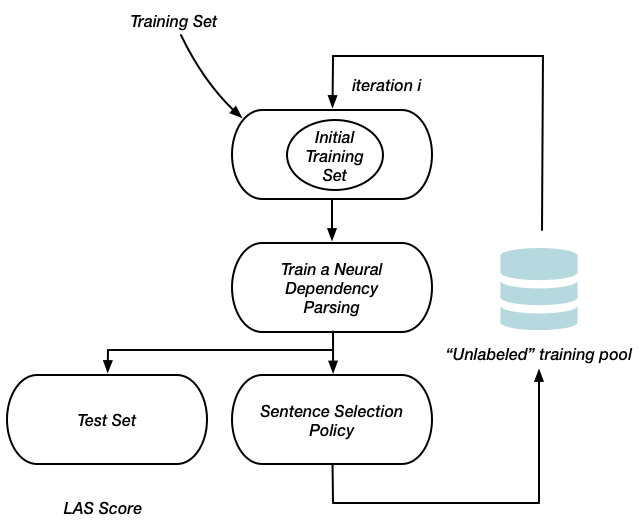
\includegraphics[width=\linewidth]{active-arch.png}
\caption{Active Learning Implementation Architecture}
\label{fig:2}
\end{figure}

We implement four sample selection policies: \emph{Random}, \emph{Length}, \emph{Raw}, and \emph{Margin}. \emph{Random} policy
asks the system to choose a random set of sentences from the ``unlabeled" training pool. \emph{Length} chooses the batch based on
the sentence length (i.e., number of words within a sentence). Intuition for this policy is that 
long sentences are usually more syntactically complex and so their parses are inevitably less certain. 
We first parse the ``unlabeled" training pool and both \emph{Raw} and \emph{Margin} select the sentences
with lowest probabilities. The lower the probability, the higher the uncertainty. By obtaining feedback on the cases 
in which the parser is most uncertain, the parser hopes to learn more than obtaining labels on random sentences in which 
its existing model is perhaps already quite confident in, and from which it would therefore not learn much. 
\emph{Raw} selects sentences based on \emph{normalized} raw probability, which is calculated by taking 
the product of the probability assigned to every transition taken to get that parse.
\emph{Margin} select sentences based on \emph{normalized} margin probability, which is done by
taking the product of the margin between probabilities assigned to two top transitions at every step. 
\emph{Normalized} means taking $2n$th ($n$ is the length of sentence) root of probabilities to compensate the fact
that longer sentences have lower probabilities due to more shift-reduce decisions that the parser has to make.

\section{Experiments and Analysis}
\label{ssec:layout}

We extract first 50 sentences from section 00 to form our initial training set. For the ``unlabeled" training set, 
we concatenate sections 01-03 of WSJ, which gives us 4485 potential training sentences (107272 words). For test set,
we use WSJ section 20. In each iteration, we use policy to select approximate 1500 words of additional training data
from ``unlabeled" training set. All the experiements are performed on
a machine that has 4 Intel(R) Core(TM) i5-6200U CPU @ 2.30GHz processors and 4GB of memory. 
We run parser for 20 iterations and we set \texttt{maxIter}, the number of training iterations to complete before stopping
and saving the final model, to be 500. The rest configuration of neural dependency parser takes \fnurl{default 
values}{https://nlp.stanford.edu/software/nndep.shtml}.
Experiment result is shown in Table \ref{valid} and corresponding learning curves are shown in Figure \ref{fig:curve}.
The commands along with the parameters for the program 
to reproduce the experiment can be found in \texttt{Makefile} shipped with the writeup.

\begin{figure}
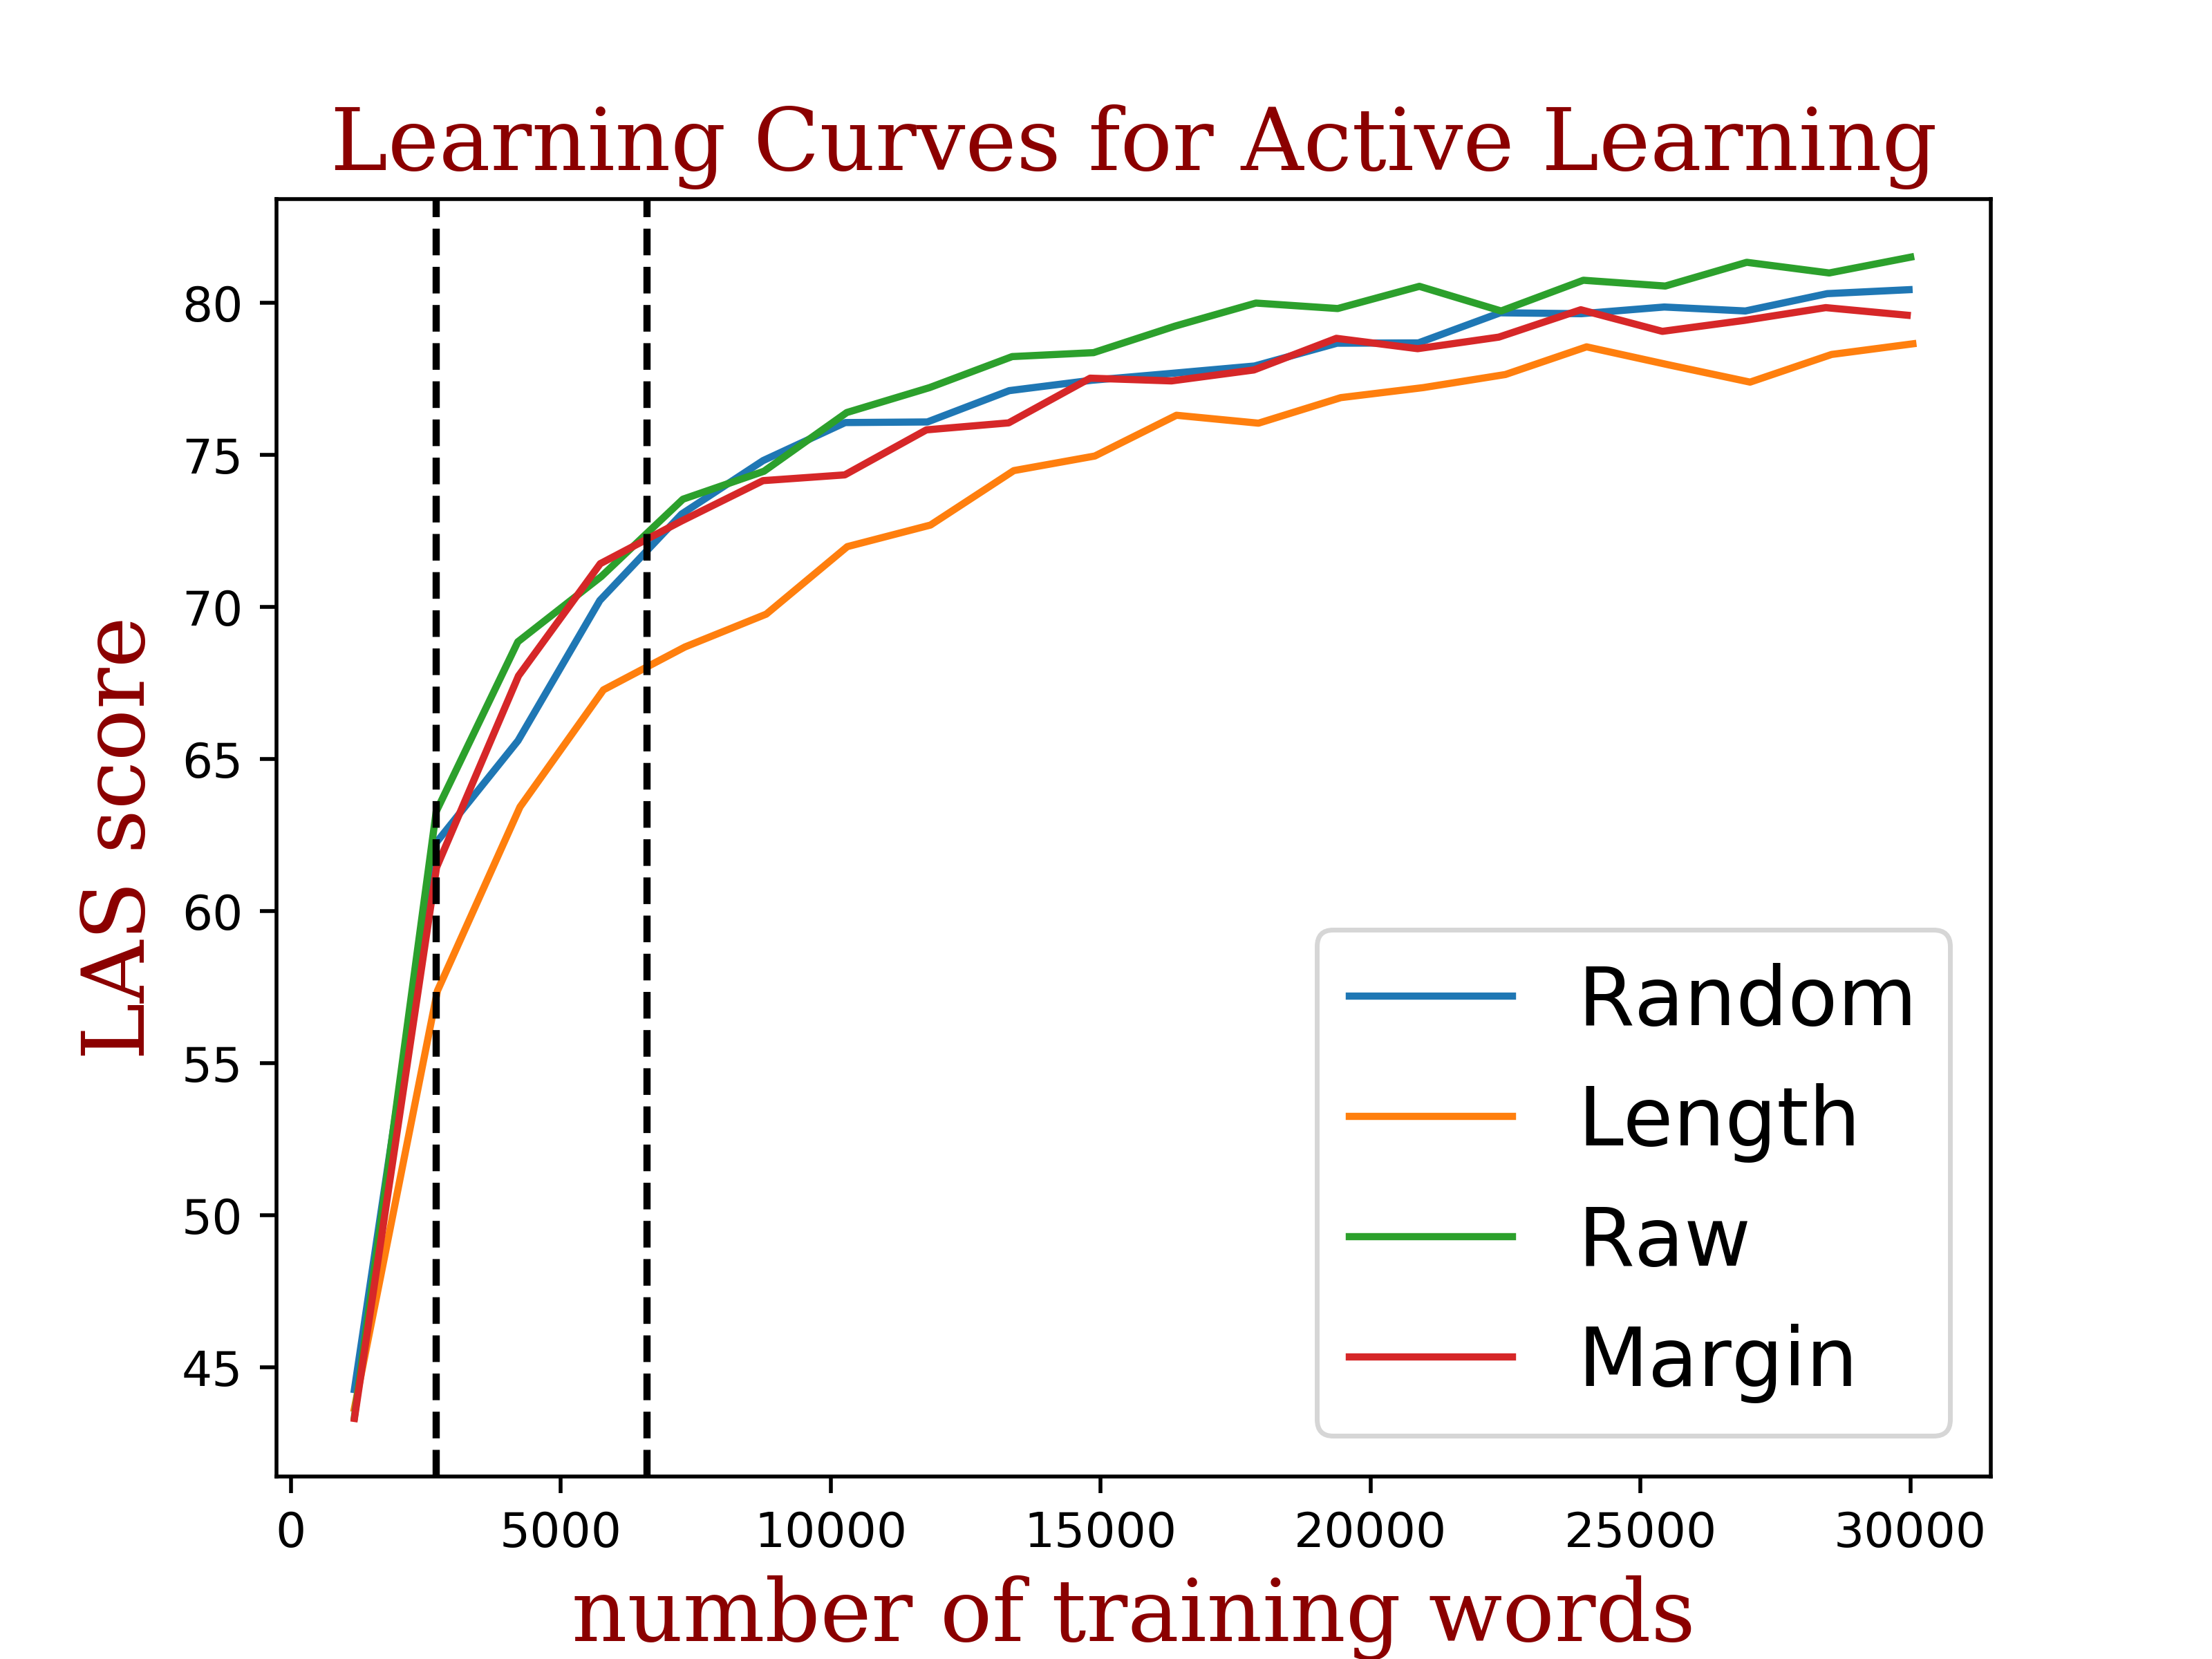
\includegraphics[scale=0.7]{curve.png}
\caption{Learning Curves for Sample Selection Policies}
\label{fig:curve}
\end{figure}

\begin{table}[]
\centering
\begin{tabular}{|l|l|l|l|}
\hline
Policy & LAS   & Training Time (s) & Training Set (words)\\ \hline\hline
Random & 80.44 & \textbf{19393} (0) &  29976 \\ \hline
Length & 78.66 & 19805 (+412)  & \textbf{30047} \\ \hline
Raw    & \textbf{81.51} & 20408 (+1015) & 30006\\ \hline
Margin & 79.60 & 19564 (+171)  & 29942 \\ \hline
\end{tabular}
\caption{Sample Selection Policy Performance}
\label{valid}
\end{table}

%\begin{table}
%\captionsetup{size=footnotesize}
%%\setlength\tabcolsep{0pt} % let LaTeX compute intercolumn whitespace
%\footnotesize\centering
%%This table provides the frequencies.
%
%\smallskip 
%\begin{tabular*}{\columnwidth}{@{\extracolsep{\fill}}lc}
%\toprule
%  Description  & Values  \\
%\midrule
% batch size & 128      \\
% number of epochs & 6 \\
% embedding size for word ID & 300        \\
% embedding size for orthographic features & 10        \\
% optimizer learning rate & 0.0005 \\
% optimizer & Adam \\
%\bottomrule
%\end{tabular*}
%\caption{BiLSTMs Configuration} \label{tab:freq}
%\end{table}

% Do the active learning methods perform better than random selection of training examples? Why?
% How do the different methods for measuring uncertainty perform compared to each other? Try to explain any observed differences between methods.
From the result, we see that \emph{Raw} outperforms \emph{Random} selection policy while \emph{Margin} and \emph{Length}
stay below \emph{Random} performance. To further verify the observation, another set of experiments is run and we have
\emph{Random}: 79.43, \emph{Length}: 78.78, \emph{Raw}: 81.40, and \emph{Margin}: 80.41. We see that \emph{Raw} is still
the best policy, \emph{Random} and \emph{Margin} stay relative close, and \emph{Length} be the worst policy. If we take a look
at learning curves, we find that active learning policies perform better than random selection in terms of learning rate. The good
performance of \emph{Raw} indicates that actively select most uncertain training sentences can truly improve
the parsing performance both in terms of final LAS score and the learning rate, which majorly because of picking sentences
that have highest learning values.

When comparing different policies for measuring uncertainty, we see that \emph{Length} is not a good policy.
This is probably becasue of two reasons. First, there is no strong correlation between the length of
the sentence and the uncertainty of the parses. Some sentences may be long but their syntactic structure might be simple. Another
possible reason is that the parser is trained bias towards long, complex sentences and fail to learn the short, simple sentences.
Overall, \emph{Length} policy leads to an offline training scheme in the sense that all the training batches can be predetermined:
the parser performance on the current batch has no impact on how the next batch of sentences should be selected. \emph{Random} and
\emph{Margin} stay very close to each other possibly due to the fact that \emph{Random} already picks the sentence with the most
gradient from a pool of random-selected sentences, which makes \emph{Random} effectly perform active learning on the provided batch.
If we take a look at Figure \ref{fig:2}, we can see that both \emph{Margin} and \emph{Raw} outperforms \emph{Random} around 5000 words,
which suggests that both \emph{Margin} and \emph{Raw} learn much more from sentences they intentionally pick than \emph{Random} that
select sentences randomly. When compare \emph{Margin} with \emph{Raw}, we can see that \emph{Raw} is a better metric of uncertainty.
Imagine a sentence with two words. The first word's action is very certain with probability 1 and the second word's actions are distributed
as 0.6 and 0.4 for the top two. Then, under \emph{Raw} policy, this sentence's probability is $1 \times 0.6 = 0.6$ while for \emph{Margin},
it is $1 \times 0.2 = 0.2$. Under \emph{Raw}, this sentence is fairly certain while for \emph{Margin}, this sentence is very uncertain. However,
as one can see, parser is only unsure about the last action but the top action is still above 0.5, which is fairly certain. However, the
parser's uncertainty get exaggerated under \emph{Margin} policy. In other words, the low margin probability may not be a good indicator
to the uncertainty of the whole parsing, which means the sentence falsely pick the sentence that has few learning value.

% Does active learning help across the complete learning curve, or are there parts of the learning curve where it performs best? Why?
If we take a closer look at the learning curve, we can see that active learning is most helpful when the number of training words between
2694 and 6600 as shown in dot lines in Figure \ref{fig:2}. Within the region, the LAS score of both \emph{Margin} and \emph{Raw} outperforms
\emph{Random}. The reason for this phenomenon is that the parser learns more from the sentences selected by the active learning policies than
by random. After 6600 number of training words, \emph{Raw} still outperforms \emph{Random} but the gap between them gets closer. One possible
explanation is that the ``unlabeled" training pool gets smaller and even by \emph{Random}, the sentences that have high learning values will
be selected with higher and higher chances. Thus, the gain from active learning gets decreased.

% How do your results compare to those presented by Hwa (2000)? Try to explain any differences.
When compare our result with Hwa \shortcite{Hwa:2000:SSS:1117794.1117800}'s experiemts' results, we can see that our experiement is closest 
to Hwa's first experiment setup, which experiments with different sample selection policy from an abundant supply of unlabeled data. When we
compare results with Hwa's, we find that both experiments show that \emph{Length} policy is less helpful. In addition, active learning
policies have faster learning rate (i.e., the slope of learning curves) than the baseline. Hwa's result shows that tree entropy is the most
effective selection policy while ours is \emph{Random}, which share same intuition about measuring uncertainty from probabilistic point of view.
Our result is different from Hwa's result in terms of difference among \emph{Random}, \emph{Length}, and \emph{Raw} performances. Hwa shows
that on average the score of \emph{Random} and \emph{Length} are the same. One furture work is to show whether Hwa's result holds in our case
when we repeatedly run several trails of our experiments. Additionaly, Hwa's result shows they can use much less \emph{brackets} when using
tree entropy policy. It seems to suggest that tree entropy is a better uncertainty measurement than \emph{Raw}. This may be true because
tree entropy is calculated by considering all possible parses while \emph{Raw} considers only the most probable parsing.

\section{Conclusion and Future Work}
\label{ssec:first}

In this writeup, we show that given a fixed amount of unlabeled training examples, active learning strategy can learn much more than 
the random selection baseline. We compare different ways of measuring uncertainty about training examples and show that \emph{Random}
policy performs the best. In the future, we may explore the composition of test set to see if parser can have great performance
on long sentences while have subpar performance on short sentence to explore the root cause of failure of \emph{Length} policy.
\bibliography{emnlp2016}
\bibliographystyle{emnlp2016}

\end{document}
